\begin{figure}[htbp]
\centering
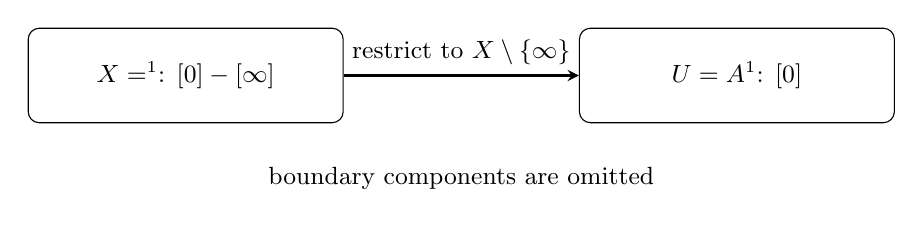
\begin{tikzpicture}[>=stealth,every node/.style={font=\small}]
\node[draw,rounded corners,minimum width=4cm,minimum height=1.2cm] (x) at (0,0) {$X=\PP^1$: $[0]-[\infty]$};
\node[draw,rounded corners,minimum width=4cm,minimum height=1.2cm] (u) at (7,0) {$U=\mathbb{A}^1$: $[0]$};
\draw[->,thick] (x)--node[above]{restrict to $X\setminus\{\infty\}$}(u);
\node at (3.5,-1.3) {boundary components are omitted};
\end{tikzpicture}
\caption{Restriction of a Weil divisor to an open subset forgets prime components contained in the boundary.}
\label{fig:vi39-restriction}
\end{figure}